%% ============================================================
%% RoboFest 6.0 -- AUV Simulation & Mapping Documentation
%% Scope: simulation environment + mapping/localisation only.
%% Object detection is covered in a companion document.
%% Compile: ./compile.sh   (runs pdflatex twice)
%% ============================================================
\documentclass[11pt,a4paper]{article}

%% ── Packages ──────────────────────────────────────────────
\usepackage[T1]{fontenc}
\usepackage[utf8]{inputenc}
\usepackage{libertinus}
\usepackage{montserrat}
\usepackage{microtype}
\usepackage[margin=2.3cm,top=2.6cm,bottom=2.8cm]{geometry}
\usepackage{graphicx}
\usepackage{xcolor}
\usepackage{amsmath,amssymb}
\usepackage{booktabs}
\usepackage{array}
\usepackage{tabularx}
\usepackage{calc}
\usepackage{colortbl}
\usepackage{enumitem}
\usepackage{listings}
\usepackage{caption}
\usepackage{tikz}
\usetikzlibrary{arrows.meta,positioning,calc}
\usepackage{hyperref}
\usepackage{fancyhdr}
\usepackage{titlesec}
\usepackage{float}
\usepackage{fontawesome5}
\usepackage[most]{tcolorbox}
\usepackage{setspace}

%% ── Palette (restrained: ink + one accent; red is reserved
%%    exclusively for "add image" call-outs, never decorative) ──
\definecolor{ink}{HTML}{16233A}
\definecolor{inksoft}{HTML}{4A5568}
\definecolor{accent}{HTML}{1B6FA8}
\definecolor{accentsoft}{HTML}{EAF3FA}
\definecolor{hairline}{HTML}{D8DEE6}
\definecolor{paper}{HTML}{FFFFFF}
\definecolor{needred}{HTML}{C0392B}
\definecolor{needredbg}{HTML}{FDEDEC}
\definecolor{tablehead}{HTML}{F3F5F7}
\definecolor{codebg}{HTML}{F5F6F8}

\hypersetup{
  colorlinks=true, linkcolor=accent, urlcolor=accent, citecolor=accent,
  pdftitle={AUV Simulation and Mapping Documentation -- RoboFest 6.0},
  pdfauthor={AUV Team}, bookmarksnumbered=true,
}

%% ── Section styling ───────────────────────────────────────
\titleformat{\section}
  {\normalfont\fontfamily{Montserrat-TLF}\selectfont\Large\bfseries\color{ink}}
  {\thesection}{0.6em}{}
  [\vspace{2pt}\textcolor{accent}{\rule{\linewidth}{1.1pt}}\vspace{2pt}]
\titlespacing*{\section}{0pt}{1.4em}{0.7em}
\titleformat{\subsection}
  {\normalfont\fontfamily{Montserrat-TLF}\selectfont\large\bfseries\color{ink}}
  {\thesubsection}{0.6em}{}
\titlespacing*{\subsection}{0pt}{1.0em}{0.4em}
\titleformat{\subsubsection}
  {\normalfont\fontfamily{Montserrat-TLF}\selectfont\normalsize\bfseries\color{inksoft}}
  {}{0em}{}
\titlespacing*{\subsubsection}{0pt}{0.8em}{0.3em}

%% ── Page style ────────────────────────────────────────────
\pagestyle{fancy}\fancyhf{}
\renewcommand{\headrulewidth}{0pt}
\renewcommand{\footrulewidth}{0.5pt}
\fancyfoot[L]{\footnotesize\color{inksoft}AUV Simulation \& Mapping Documentation}
\fancyfoot[R]{\footnotesize\color{inksoft}\thepage}
\fancypagestyle{plain}{\fancyhf{}\renewcommand{\headrulewidth}{0pt}
  \fancyfoot[L]{\footnotesize\color{inksoft}AUV Simulation \& Mapping Documentation}
  \fancyfoot[R]{\footnotesize\color{inksoft}\thepage}}

%% ── Listings (single restrained style) ───────────────────
\lstdefinestyle{cleanbash}{
  backgroundcolor=\color{codebg}, basicstyle=\ttfamily\small\color{ink},
  keywordstyle=\color{accent}\bfseries, commentstyle=\color{inksoft}\itshape,
  numbers=none, frame=single, framesep=6pt, rulecolor=\color{hairline},
  breaklines=true, captionpos=b, xleftmargin=8pt, framexleftmargin=8pt,
  language=bash,
}

%% ── tcolorbox call-outs ───────────────────────────────────
\tcbuselibrary{skins,breakable}
\newtcolorbox{infobox}[1][]{
  colback=accentsoft, colframe=accent, coltitle=ink, boxrule=0.8pt,
  fonttitle=\fontfamily{Montserrat-TLF}\bfseries, title={Note}, rounded corners, #1}
\newtcolorbox{keybox}[1][]{
  colback=ink!4, colframe=ink, coltitle=white, boxrule=0.8pt,
  fonttitle=\fontfamily{Montserrat-TLF}\bfseries, title={At a Glance}, rounded corners, #1}

%% ── Table helpers ─────────────────────────────────────────
\newcolumntype{C}[1]{>{\centering\arraybackslash}p{#1}}
\newcolumntype{L}[1]{>{\raggedright\arraybackslash}p{#1}}
\renewcommand{\arraystretch}{1.35}

%% ── Shortcuts ─────────────────────────────────────────────
\newcommand{\code}[1]{\texttt{\small\color{accent}#1}}
\setlength{\parskip}{4pt}
\setlength{\parindent}{0pt}
\newcommand{\nl}{\newline}

%% ── Red "add image" call-out block ───────────────────────
%% Usage: \imageneeded[width]{filename}{Title}{What to capture, and how}
\newcommand{\imageneeded}[4][0.86\textwidth]{%
  \IfFileExists{photos/#2}{%
    \begin{figure}[H]\centering
      \includegraphics[width=#1,keepaspectratio]{photos/#2}
    \end{figure}
  }{%
    \begin{center}
    \fboxsep=10pt
    \fcolorbox{needred}{needredbg}{%
      \begin{minipage}{#1-2\fboxsep}\centering
        \vspace{7pt}
        {\large\color{needred}\faCameraRetro}\\[4pt]
        {\fontfamily{Montserrat-TLF}\bfseries\large\color{needred}ADD IMAGE -- #3}\\[4pt]
        {\small\color{needred}#4}\\[4pt]
        {\footnotesize\ttfamily\color{inksoft}save as: docs/photos/#2}
        \vspace{7pt}
      \end{minipage}}
    \end{center}
  }%
}

\begin{document}

%% ════════════════════════ COVER ══════════════════════════
\begin{titlepage}
\pagecolor{ink}\color{white}
\begin{center}
\vspace*{1.2cm}
\textcolor{accent}{\rule{\textwidth}{2pt}}
\vspace{0.5cm}

{\fontfamily{Montserrat-TLF}\selectfont\small\bfseries\color{accent!70!white}
  ROBOFEST 6.0 \ \textbar\ \ AUTONOMOUS UNDERWATER VEHICLE}

\vspace{0.6cm}
{\fontfamily{Montserrat-TLF}\selectfont\fontsize{34}{40}\bfseries\selectfont SIMULATION}\\[1pt]
{\fontfamily{Montserrat-TLF}\selectfont\fontsize{34}{40}\bfseries\selectfont\textcolor{accent}{\& MAPPING}}

\vspace{0.4cm}
\textcolor{accent!60!white}{\rule{0.5\textwidth}{0.6pt}}
\vspace{0.45cm}

{\large\color{white!85!black} Simulation Environment, System Architecture,\\
Mission Navigation \& Mapping Pipeline}

\vspace{0.9cm}
\imageneeded[0.56\textwidth]{00-auv-hero.jpg}{AUV Hero Shot}
  {Simulation or real photo of the AUV, used as the cover image.}

\vspace{0.9cm}
\begin{tabular}{rl}
  \textcolor{accent!70!white}{\textbf{Competition:}} & RoboFest 6.0 \\[3pt]
  \textcolor{accent!70!white}{\textbf{Document:}} & Simulation \& Mapping Technical Report \\[3pt]
  \textcolor{accent!70!white}{\textbf{Simulator:}} & Gazebo Harmonic + ROS\,2 Jazzy \\[3pt]
  \textcolor{accent!70!white}{\textbf{Date:}} & \today \\
\end{tabular}

\vspace{0.8cm}
\textcolor{accent}{\rule{\textwidth}{2pt}}
\vspace{0.4cm}

{\footnotesize\color{white!55!black}\itshape
Object detection (YOLO training, dataset, metrics) is covered in a separate\\
Object Detection Documentation, to be combined with this report at final submission.}
\end{center}
\end{titlepage}
\pagecolor{white}\color{black}

%% ── Contents ──────────────────────────────────────────────
\thispagestyle{plain}
\tableofcontents
\clearpage

%% ════════════════════════ 1. EXEC SUMMARY ═══════════════
\section{Executive Summary}

This report documents the simulation environment, system architecture, navigation
behaviour, and mapping pipeline built for an Autonomous Underwater Vehicle (AUV)
competing in \textbf{RoboFest 6.0}. The full software stack runs on \textbf{ROS\,2 Jazzy}
inside a \textbf{Gazebo Harmonic} simulated pool, and is designed so that moving to
real hardware requires only a configuration change, not a code change.

\begin{keybox}
\begin{itemize}[noitemsep,leftmargin=1.4em]
  \item Full three-phase mission: gate crossing (round trip) $\to$ green zone
    acquisition $\to$ blue bin hold.
  \item Ground-truth odometry at 50\,Hz, with a trail-mapping node that records and
    visualises the AUV's trajectory live in RViz2.
  \item Every tunable value lives in \code{sim\_params.yaml}; no source-code changes
    are needed when moving to real hardware.
  \item Single-command launch: \code{ros2 launch auv\_bringup sim\_mission.launch.py}.
\end{itemize}
\end{keybox}

\textbf{Scope of this document.} This report covers the \emph{simulation
environment, system integration, mission navigation, and mapping/localisation}.
Object detection (YOLO model training, dataset preparation, HSV tuning,
detection accuracy) is developed and documented separately by the perception
team; the two reports will be combined into a single submission package.

%% ════════════════════════ 2. MISSION OVERVIEW ═══════════
\section{Mission Overview}

The AUV executes a single continuous, fully autonomous mission in three phases:

\begin{enumerate}[leftmargin=1.6em]
  \item \textbf{Gate Navigation} -- search for, approach, align with, and cross an
    underwater gate, then repeat the crossing on the return leg.
  \item \textbf{Green Zone Acquisition} -- locate a green target mat on the pool
    floor and hold position above it.
  \item \textbf{Blue Bin Hold} -- locate a blue bin on the mat and hold position
    above it to close out the mission.
\end{enumerate}

\begin{figure}[H]
\centering
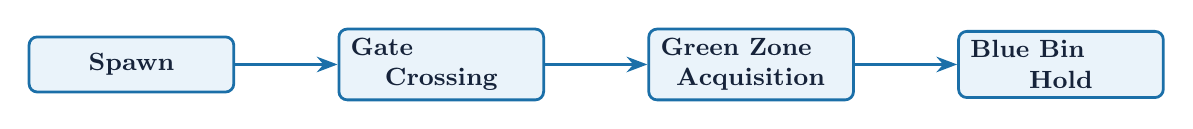
\begin{tikzpicture}[scale=0.92,
  box/.style={rectangle,rounded corners=3pt,minimum width=2.6cm,minimum height=0.7cm,
    text width=2.3cm,align=center,font=\small\bfseries,draw=accent,line width=1pt,fill=accentsoft,text=ink},
  arr/.style={-Stealth,color=accent,line width=1pt},
]
  \node[box] (a) {Spawn};
  \node[box,right=1.3cm of a]  (b) {Gate\nl Crossing};
  \node[box,right=1.3cm of b]  (c) {Green Zone\nl Acquisition};
  \node[box,right=1.3cm of c]  (d) {Blue Bin\nl Hold};
  \draw[arr] (a)--(b); \draw[arr] (b)--(c); \draw[arr] (c)--(d);
\end{tikzpicture}
\caption{Mission phase flow: gate round trip, then green zone, then blue bin hold.}
\end{figure}

%% ════════════════════════ 3. SIMULATION ENV ═══════════════
\section{Simulation Environment}

\subsection{Gazebo World}

The mission is simulated in Gazebo Harmonic, chosen for native ROS\,2
integration, full 6-DOF rigid-body physics, and high-fidelity stereo camera
simulation. The world file (\texttt{camera\_test.sdf}) places the gate, green
mat, blue bin, and AUV spawn point at fixed coordinates, with zero world
gravity -- the AUV holds depth through its motion plugin rather than buoyancy
in this phase.

\begin{table}[H]
\centering
\caption{Key world elements}
\begin{tabularx}{\textwidth}{L{3.2cm} L{3.4cm} X}
  \toprule
  \rowcolor{tablehead}\textbf{Element} & \textbf{Position} & \textbf{Description} \\
  \midrule
  Gate            & $(0, 12, -4.5)$   & Vertical poles + crossbar \\
  Green mat       & $(10, 22, -5.0)$  & Target zone on pool floor \\
  Blue bin        & $(10, 22, -4.75)$ & Sits on the green mat \\
  AUV spawn       & $(-5, 0, z_d)$    & Configurable via launch arguments \\
  \bottomrule
\end{tabularx}
\end{table}

\imageneeded{01-gate-world.png}{Gate in Gazebo}
  {Overhead or angled Gazebo screenshot showing the gate structure clearly.}

\imageneeded{02-mat-bin-world.png}{Green Mat \& Blue Bin}
  {Gazebo screenshot of the green target mat with the blue bin resting on it.}

\subsection{AUV Vehicle Model}

The vehicle model (\texttt{auv\_box}) is built from the design team's CAD export
and carries realistic mass and inertia properties.

\begin{table}[H]
\centering
\caption{AUV physical properties}
\begin{tabular}{L{5cm} C{3cm} L{4.6cm}}
  \toprule
  \rowcolor{tablehead}\textbf{Property} & \textbf{Value} & \textbf{Notes} \\
  \midrule
  Bounding box  & $0.92\times0.83\times0.58$\,m & Collision geometry \\
  Mass          & 11.74\,kg & Design team CAD value \\
  Visual mesh   & \texttt{base\_link.STL} & SolidWorks export \\
  \bottomrule
\end{tabular}
\end{table}

\imageneeded{03-auv-model.png}{AUV Vehicle}
  {Gazebo screenshot of the AUV model, and/or a photo of the real vehicle.}

\subsection{Sensor Suite}

The AUV carries three cameras modelled after the OAK-D Lite: a front stereo
pair (0.075\,m baseline) for depth estimation and gate localisation, and a
downward-facing bottom camera for close-range zone centring.

\begin{table}[H]
\centering
\caption{Camera specifications}
\begin{tabular}{L{4.2cm} L{3.4cm} L{5cm}}
  \toprule
  \rowcolor{tablehead}\textbf{Parameter} & \textbf{Value} & \textbf{Notes} \\
  \midrule
  Resolution      & $640\times480$\,px & All three cameras \\
  Horizontal FOV  & $\approx73^\circ$  & OAK-D Lite spec \\
  Update rate     & 15\,Hz             & All cameras \\
  Range           & 0.2 -- 19.1\,m     & Near / far clip planes \\
  Stereo baseline & 0.075\,m           & Front pair, centre-to-centre \\
  \bottomrule
\end{tabular}
\end{table}

\subsection{Motion \& Physics}

In this phase the AUV is driven by a kinematic velocity-control plugin
(perfect velocity tracking, no thruster tuning required), which decouples
navigation development from thruster dynamics. Hydrodynamic drag
coefficients (Fossen model, BlueROV2 basis) are pre-configured in the world
file and activate automatically once thruster allocation is implemented,
without any change to the navigation logic.

%% ════════════════════════ 4. ARCHITECTURE ═══════════════
\section{System Architecture}

\subsection{Workspace Layout}

\begin{lstlisting}[style=cleanbash, caption={AUV workspace structure (active packages)}]
~/auv_ws/
|-- src/
|   |-- auv_planner/       # Mission FSMs: gate + green navigators
|   |-- auv_vision/        # Perception nodes (see companion doc)
|   |-- auv_telemetry/     # CSV logger, dashboard, trail mapper
|   |-- auv_description/   # SDF model, meshes, launch, RViz config
|   `-- auv_bringup/       # Top-level launch + sim_params.yaml
|-- camera_test.sdf        # Gazebo world file
`-- mission_logs/          # Auto-created CSV and trail logs
\end{lstlisting}

\subsection{ROS\,2 -- Gazebo Bridge}

All Gazebo topics are bridged into the \texttt{/auv/} ROS\,2 namespace, so
downstream nodes never reference Gazebo-specific topic names directly.

\begin{table}[H]
\centering
\caption{Core bridged topics}
\begin{tabular}{L{5.6cm} L{3.4cm} C{1.6cm}}
  \toprule
  \rowcolor{tablehead}\textbf{Topic} & \textbf{Type} & \textbf{Dir.} \\
  \midrule
  \texttt{.../left/image\_raw}   & Image    & GZ$\to$ROS \\
  \texttt{.../right/image\_raw}  & Image    & GZ$\to$ROS \\
  \texttt{.../bottom/image\_raw} & Image    & GZ$\to$ROS \\
  \texttt{odometry} $\to$ \texttt{/auv/odom} & Odometry & GZ$\to$ROS \\
  \texttt{cmd\_vel}              & Twist    & ROS$\to$GZ \\
  \bottomrule
\end{tabular}
\end{table}

\subsection{Node Graph}

\begin{figure}[H]
\centering
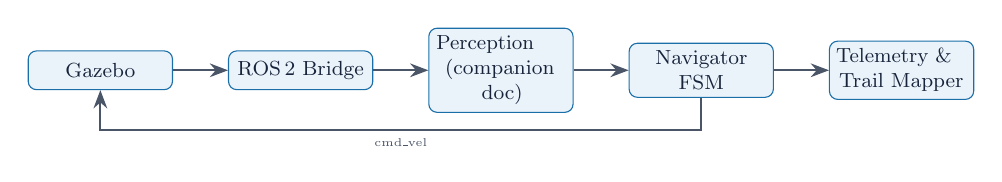
\begin{tikzpicture}[scale=0.82,every node/.append style={scale=0.82},
  node distance=0.5cm and 0.7cm,
  n/.style={rectangle,rounded corners=3pt,fill=accentsoft,draw=accent,
    minimum width=2.2cm,minimum height=0.6cm,text width=2.0cm,
    align=center,font=\small,text=ink},
  arr/.style={-Stealth,line width=0.8pt,color=inksoft},
]
  \node[n] (gz) {Gazebo};
  \node[n,right=of gz] (br) {ROS\,2 Bridge};
  \node[n,right=of br] (pe) {Perception\nl (companion doc)};
  \node[n,right=of pe] (nv) {Navigator FSM};
  \node[n,right=of nv] (tl) {Telemetry \&\nl Trail Mapper};
  \draw[arr] (gz)--(br); \draw[arr] (br)--(pe); \draw[arr] (pe)--(nv);
  \draw[arr] (nv)--(tl);
  \draw[arr] (nv.south)--+(0,-0.5)-|node[below,font=\tiny,inksoft,pos=0.25]{cmd\_vel}(gz.south);
\end{tikzpicture}
\caption{High-level data flow. Perception detail is covered in the companion document.}
\end{figure}

%% ════════════════════════ 5. NAVIGATION ═══════════════
\section{Mission Navigation}

The navigator nodes consume 3D object positions published by the perception
pipeline (over well-defined \texttt{/auv/} topics) and convert them into
velocity commands. This section covers only that navigation and control
behaviour -- the detection algorithms themselves are documented separately.

\subsection{Gate Navigation}

The gate is crossed on both the forward and return legs using a search
$\to$ track $\to$ align $\to$ cross sequence, repeated in reverse for the
return trip. The gate's position is stored in the world-fixed odometry
frame (not the camera frame), which lets the AUV keep navigating toward it
even during the brief periods when it is out of camera view.

\begin{table}[H]
\centering
\caption{Gate navigation sequence}
\begin{tabular}{L{2.6cm} L{9.8cm}}
  \toprule
  \rowcolor{tablehead}\textbf{Stage} & \textbf{Behaviour} \\
  \midrule
  Search  & Sweep laterally until the gate is detected \\
  Track   & Drive toward the gate, refining its 3D position \\
  Align   & Rotate to face the gate opening squarely \\
  Cross   & Drive straight through, then repeat in reverse for the return leg \\
  \bottomrule
\end{tabular}
\end{table}

\imageneeded{04-gate-crossing.png}{AUV Crossing the Gate}
  {Gazebo screenshot of the AUV mid-crossing through the gate opening.}

\subsection{Green Zone \& Blue Bin}

After the gate round trip, the navigator switches to a search $\to$ approach
$\to$ centre sequence over the green mat, then repeats a shorter approach
over the blue bin before holding position to close out the mission.

\begin{keybox}[title={Robustness Notes}]
\begin{itemize}[noitemsep,leftmargin=1.4em]
  \item Stored target coordinates are frozen once the AUV is very close, since
    bounding-box centres become unreliable at short range.
  \item Any single position update that jumps implausibly far is discarded,
    protecting the stored target from a single bad detection frame.
  \item If detections go briefly stale, the navigator falls back to odometry
    dead-reckoning toward the last known target position.
\end{itemize}
\end{keybox}

%% ════════════════════════ 6. MAPPING ══════════════════════
\section{Mapping \& Localisation}

\subsection{Odometry-Based Localisation}

Gazebo's odometry plugin publishes ground-truth 6-DOF pose at 50\,Hz on
\texttt{/auv/odom}, which is the single source of position and heading used
throughout the stack -- by the navigators, the telemetry logger, and the
trail mapper.

\begin{table}[H]
\centering
\caption{Odometry topic}
\begin{tabular}{L{3.4cm} L{9cm}}
  \toprule
  \rowcolor{tablehead}\textbf{Property} & \textbf{Value} \\
  \midrule
  Topic   & \texttt{/auv/odom} \\
  Rate    & 50\,Hz \\
  Frame   & \texttt{map} (world-fixed) \\
  Data    & Position, orientation, and velocity \\
  \bottomrule
\end{tabular}
\end{table}

\subsection{Trajectory (Trail) Mapping}

A dedicated trail-mapper node records the AUV's path as a \texttt{nav\_msgs/Path},
adding a new point only once the AUV has moved at least 0.10\,m, and
publishes it at 1\,Hz for live visualisation.

\begin{table}[H]
\centering
\caption{Trail mapper output}
\begin{tabular}{L{3.4cm} L{9cm}}
  \toprule
  \rowcolor{tablehead}\textbf{Property} & \textbf{Value} \\
  \midrule
  Min. point spacing & 0.10\,m \\
  Publish rate       & 1.0\,Hz \\
  Output             & \texttt{/auv/trail\_map} (RViz2) + CSV log \\
  \bottomrule
\end{tabular}
\end{table}

\imageneeded{05-rviz-trajectory.png}{RViz2 Trajectory Map}
  {RViz2 screenshot showing the recorded trail (green line) from spawn through
   the gate to the green mat, with the AUV's current pose marker.}

A pre-configured RViz2 layout renders this live: a pose arrow at the AUV's
current position and a growing trail line for the full trajectory, on a
world-fixed \texttt{map} frame with a dark background for underwater
readability.

\subsection{Sim-to-Real Localisation}

\begin{table}[H]
\centering
\caption{Localisation: simulation vs.\ real hardware}
\begin{tabular}{L{3cm} L{4.6cm} L{4.8cm}}
  \toprule
  \rowcolor{tablehead}\textbf{Component} & \textbf{Simulation} & \textbf{Real Hardware} \\
  \midrule
  Position & Gazebo odometry (ground truth) & EKF fusing DVL + IMU \\
  Heading  & Gazebo quaternion (perfect)     & IMU magnetometer \\
  Mapping pipeline & \multicolumn{2}{c}{Identical -- same trail mapper and RViz2 config} \\
  \bottomrule
\end{tabular}
\end{table}

%% ════════════════════════ 7. TESTING ═══════════════
\section{Testing \& Validation}

\subsection{Nominal Mission Run}

A full simulation run is validated end-to-end against a fixed scenario:
AUV spawned at $(-5, 0, -4.238)$ facing the gate, gate at $(0, 12, -4.5)$,
green mat at $(10, 22, -5.0)$.

\begin{enumerate}[leftmargin=1.6em,itemsep=1pt]
  \item Gate round trip: search, track, align, cross, then repeat in reverse.
  \item Hand-off to the green navigator on gate completion.
  \item Green mat search, approach, and centring.
  \item Blue bin search, approach, and position hold.
  \item Mission marked complete; telemetry and trail logs finalised.
\end{enumerate}

An adversarial variant spawns the AUV off-axis (facing \emph{away} from the
gate, with a lateral offset), forcing a wide search sweep before the gate
enters camera view -- this exercises the odom-frame target tracking and
outlier rejection described in Section~5 under realistic worst-case
conditions.

\subsection{Live Monitoring Commands}

\begin{lstlisting}[style=cleanbash, caption={Useful commands during a simulation run}]
# Watch mission phase transitions live
ros2 topic echo /auv/mission_state

# Watch AUV pose and velocity
ros2 topic echo /auv/odom

# Record a full mission for later playback and analysis
ros2 bag record -a -o ~/auv_ws/mission_logs/run_bag/
\end{lstlisting}

%% ════════════════════════ 8. LAUNCH ═══════════════
\section{Launch \& Operation}

\begin{lstlisting}[style=cleanbash, caption={Full mission launch}]
source ~/auv_ws/install/setup.bash
ros2 launch auv_bringup sim_mission.launch.py

# Optional: custom spawn position
ros2 launch auv_bringup sim_mission.launch.py \
    spawn_x:=-5.0 spawn_y:=0.0 spawn_z:=-4.238 spawn_yaw:=0.0
\end{lstlisting}

A single launch file starts Gazebo, spawns the AUV, brings up the ROS\,2
bridge, and starts all mission nodes in the correct order automatically.
Mission telemetry (CSV logs and trail data) is written to
\texttt{mission\_logs/} for every run.

%% ════════════════════════ 9. LIMITATIONS ═══════════════
\section{Known Limitations \& Next Steps}

The simulation stack is deliberately built to de-risk navigation and mapping
before hardware is involved; a few gaps are already understood and planned for.

\begin{table}[H]
\centering
\caption{Current limitations and planned resolutions}
\begin{tabular}{L{3.6cm} L{4.6cm} L{4.4cm}}
  \toprule
  \rowcolor{tablehead}\textbf{Limitation} & \textbf{Impact} & \textbf{Planned Resolution} \\
  \midrule
  Kinematic velocity control & No real hydrodynamic response yet & Thruster allocation package (Phase~2) \\
  Ground-truth odometry & Won't be available on real hardware & EKF fusing DVL + IMU \\
  Planar (XY) navigation & No active depth control & Z-axis depth controller \\
  Fixed world layout & Tuned to a single gate pose & Generalise to arbitrary gate placement \\
  \bottomrule
\end{tabular}
\end{table}

None of these require changes to the mapping pipeline itself: the trail
mapper and RViz2 visualisation already consume odometry through the same
\texttt{/auv/odom} topic that the real EKF will publish to.

%% ════════════════════════ 10. CONCLUSION ═══════════════
\section{Conclusion}

This report has covered the simulation environment, system architecture,
mission navigation behaviour, and mapping/localisation pipeline for the
RoboFest 6.0 AUV. The environment models the gate, green zone, and blue bin
mission with a realistic vehicle model and camera suite; navigation executes
a robust search-track-align-cross sequence with odom-frame target tracking;
and the mapping pipeline provides full trajectory visibility through
ground-truth odometry, trail recording, and live RViz2 visualisation. All
parameters are externalised to configuration files, so the transition to
real hardware requires no change to this logic.

\begin{infobox}[title={Companion Document}]
Object detection -- model training, dataset preparation, and detection
accuracy -- is documented separately by the perception team. The two
documents will be combined into a single submission package.
\end{infobox}

\end{document}
